\documentclass[12pt]{article}
\usepackage[english]{babel}
\usepackage[utf8]{inputenc} % Permite el uso de caracteres del Español
\usepackage[T1]{fontenc}
\usepackage{graphicx}
\usepackage{amsmath}
\usepackage{wrapfig}
\usepackage{enumerate}
\usepackage[top=1in, bottom=1.25in, left=1.1in, right=1.1in]{geometry}
\usepackage[dvipsnames]{xcolor}
\usepackage{subcaption}

% Carátula del Artículo

\title{Reporte de la Actividad 4}

\author{Marco Antonio Cabello López \\ Grupo 1}

\date{Domingo 17 de Febrero del 2019}

\begin{document}
\maketitle 
\section{Introducción}
Primeramente y como introducción, en esta actividad nos enfocamos en el uso de la biblioteca Matplotlib, en un entorno de Jupyter Notebooks y en el contexto de análisis de datos. El análisis se realizo sobre los datos meteorológicos de Valle de Bravo, un municipio del estado de México, los cuales fueron proporcionados por el Servicio Meteorológico Nacional. \\
En esta actividad iniciaremos con las tareas de visualización de gráficos estadísticos con los datos diarios de precipitación, temperaturas mínimas y máximas proporcionados por el Servicio Meteorológico Nacional.    \\

\section{Desarrollo de la actividad}
\subsection{Metodología}
Se importaron las siguientes bibliotecas en el archivo de Jupyter Notebooks para trabajar con los datos de Valle de Bravo: 

\begin{center}
\textcolor{ForestGreen} {import} pandas \textcolor{ForestGreen}{as} pd\\
\textcolor{ForestGreen} {import} numpy \textcolor{ForestGreen} {as} np\\
\textcolor{ForestGreen} {import} seaborn \textcolor{ForestGreen} {as} sns\\
\textcolor{ForestGreen} {import} matplotlib.pyplot \textcolor{ForestGreen} {as} plt\\


\end{center}Estas nos ayudaran con los cálculos matemáticos, el análisis estadístico y la realización de graficas.
Después se leyó el archivo mediante el comando “pd.read\_csv”, y posteriormente se creo un Data Frame mediante el comando “pd.DataFrame()”.
Como el archivo cuenta con una columna de fechas, a esta se le dio formato de fecha mediante:

\begin{center}
\begin{verbatim}
df['FECHA'] = pd.to_datetime(df.apply(lambda x: x['FECHA'], 1)
    \end{verbatim}
\end{center}
Para elaborar las gráficas se emplearon diversas funciones sobre el Data Frame.\\
\begin{table}[]
\centering
\caption{Funciones de Data Frame empleadas.}
\begin{tabular}{|c|c|}
\hline
Función         & Acción              \\ \hline
df.head()       & Encabezado          \\ \hline
df.tail()       & Final               \\ \hline
df.dtypes()     & Tipos de variables  \\ \hline
df.mean()       & Promedio            \\ \hline
df.std()        & Desviación Estándar \\ \hline
df.median()     & Mediana             \\ \hline
df.max()        & Máximo              \\ \hline
df.min()        & Mínimo              \\ \hline
df.describe()   & Resumen estadístico \\ \hline
df.sum()         & Sumar           \\ \hline
df.shape()      & Estructurar Filas y Columnas    \\ \hline
df.index()     &  Indice     \\ \hline
df.count()     & Conteo de datos     \\ \hline
df.corr()       & Correlación       \\ \hline
df.PRECIP.max()        & Precipitación Máxima            \\ \hline
df.unique()     & Valores diferentes  \\ \hline
\end{tabular}
\end{table}Determinamos el número de años que hay en el archivo mediante el conteo de los datos, obtuvimos 54 años, los cuales se asignaron con el comando:
\begin{center}
\begin{verbatim}
init = 1961
AÑOS = [init + i for i in range(0, 54)]
PAÑO = [ df[df.AÑO==(init + i)].PRECIP.sum() for i in range(0, 54)]
    \end{verbatim}
\end{center} Para tener arreglos con dias, meses y años declaramos el de los meses de 0 a 12, y el de los años de 1961 hasta 2014. Para tener los nombres de los meses, también se creó otro arreglo:
\begin{center}
\begin{verbatim}
df['MES'] = df['FECHA'].dt.month
df['AÑO'] = df['FECHA'].dt.year
 \end{verbatim}
\end{center} Para hacer los gráficos de caja se recurrió a la biblioteca Seaborn, ya que no fue posible realizarla mediante Matplotlib.
Recurrimos a los siguientes comandos para hacerlo a partir del DataFrame:
\begin{center}
\begin{verbatim}
ax = sns.boxplot(x="AÑO", y="TMIN", data=df)
plt.xticks(rotation=45)
plt.title("Temperatura mínima promedio anual para cada año (1961-2014)")
plt.ylabel ("Temp C")
 \end{verbatim}
\end{center}

\newpage
\subsection{Resultados}
\noindent\textbf {1. Elabora una gráfica de barras (barplot) de precipitación mensual acumulada promedio de la colección de datos de la estación que se esté analizando.} \\
Podemos apreciar que los meses más lluviosos han sido Julio, Agosto y Septiembre.
\begin{center}
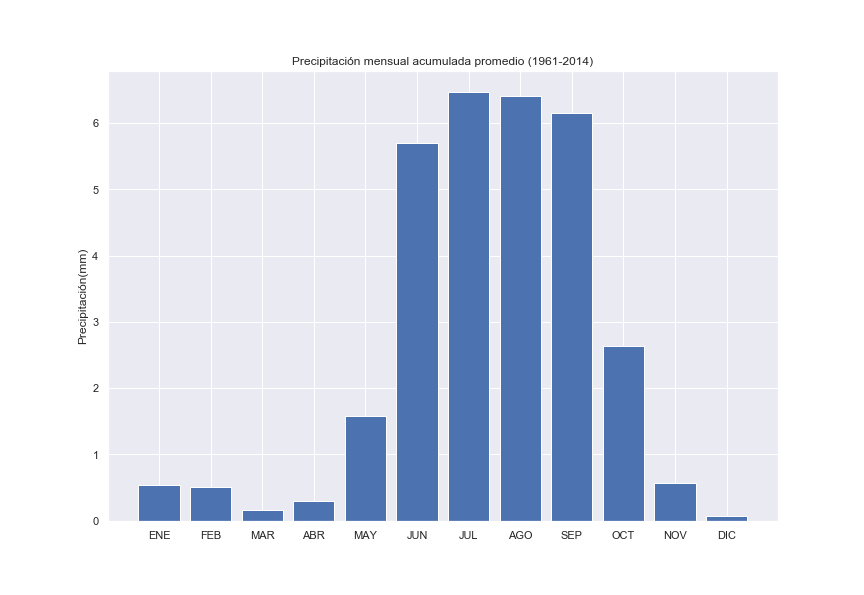
\includegraphics[scale=0.4]{Precip_men.png}
\end{center}

\noindent\textbf {2. Elabora una gráfica de barras de precipitación acumulada para cada año de la misma colección.} \\
Podemos afirmar que los años con mayores precipitaciones fueron 1957, 1973 y 2010, y que el archivo carece de datos de 1977-2000.
\begin{center}
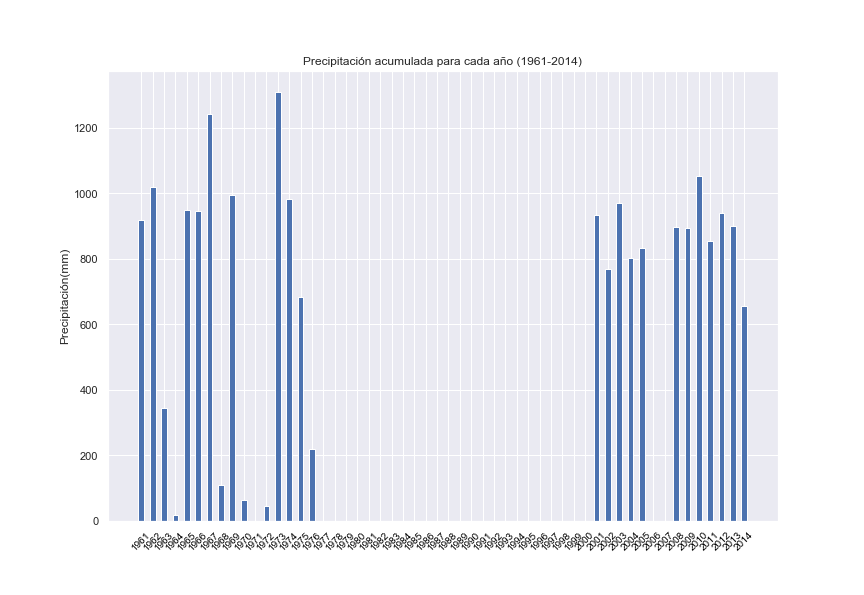
\includegraphics[scale=0.4]{Precip_anu.png}
\end{center} 

\noindent\textbf {3. Elabora una gráfica de la evolución de la temperatura máxima y mínima en la misma figura, como función del tiempo de la colección de datos.} \\
Determinamos la evolucion temporal de la temperatura máxima (amarillo) y mínima (negro) en el municipio de Valle de Bravo, notamos que la temperatura ha variado en un rango de aproximadamente 0-35ºC.
\begin{center}
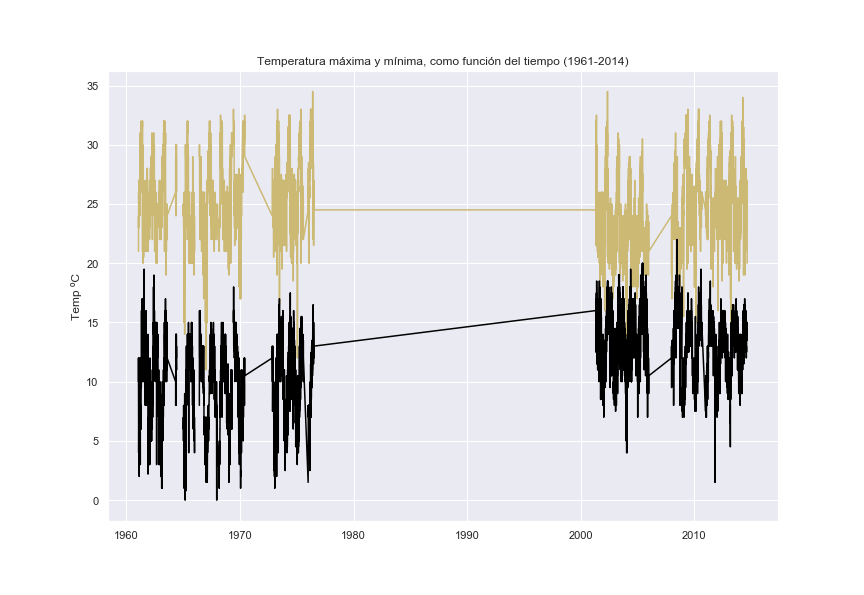
\includegraphics[scale=0.5]{Temp_maxymin.png}
\end{center} 


\noindent\textbf {4. Elabora una gráfica de cajas (boxplot) de la temperatura promedio mensual para la temperatura mínima y máxima por separado.} \\
Podemos observar que los meses de Enero, Febrero y Diciembre presentaron la menor temperatura mínima promedio, y los meses de Abril y Mayo presentaron la mayor temperatura máxima promedio.
\begin{center}
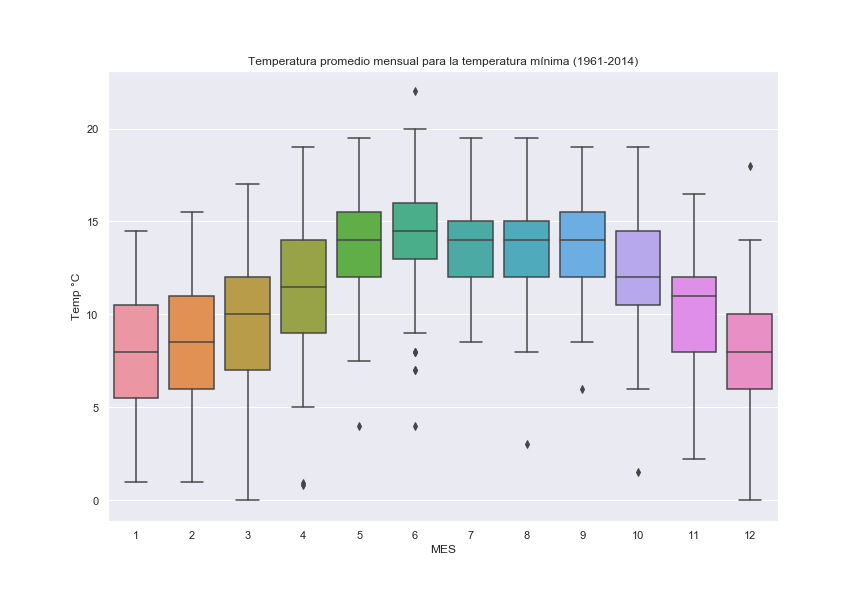
\includegraphics[height=5.3cm]{Temp_prommenmin.png}
\hspace*{\fill}
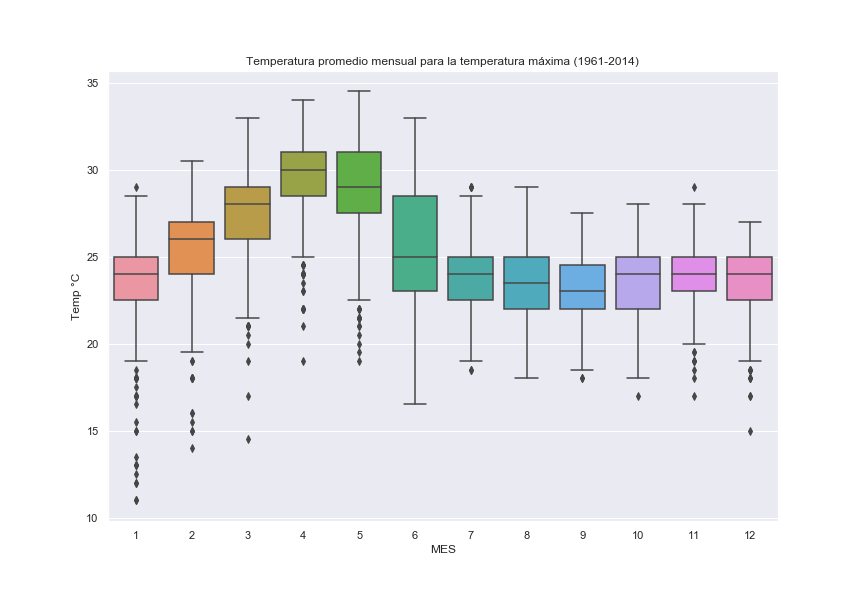
\includegraphics[height=5.3cm]{Temp_prommenmax.png}
\end{center} 




\noindent\textbf {5. Elabora una gráfica de cajas de la temperatura mínima y máxima promedio anual para cada año por separado.} \\
Podemos analizar que el año de 1970 presento la menor temperatura mínima promedio y que de 2001-2014 la temperatura mínima promedio es mayor en comparación con la temperatura mínima promedio de la época 1961-1976, y los meses de Abril y Mayo presentaron la mayor temperatura máxima promedio, además el año de 1970 presento la mayor temperatura máxima promedio.
\begin{center}
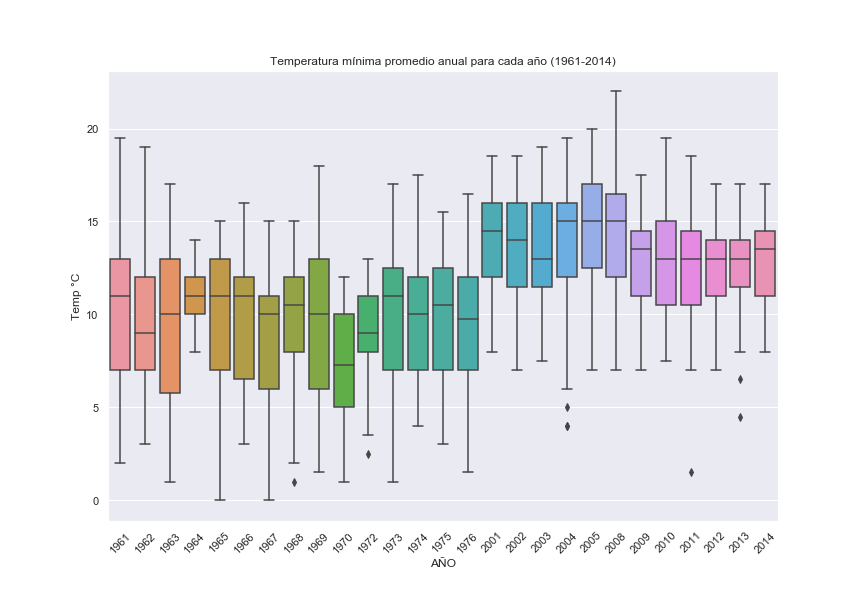
\includegraphics[height=5.3cm]{Temp_promanumin.png}
\hspace*{\fill}
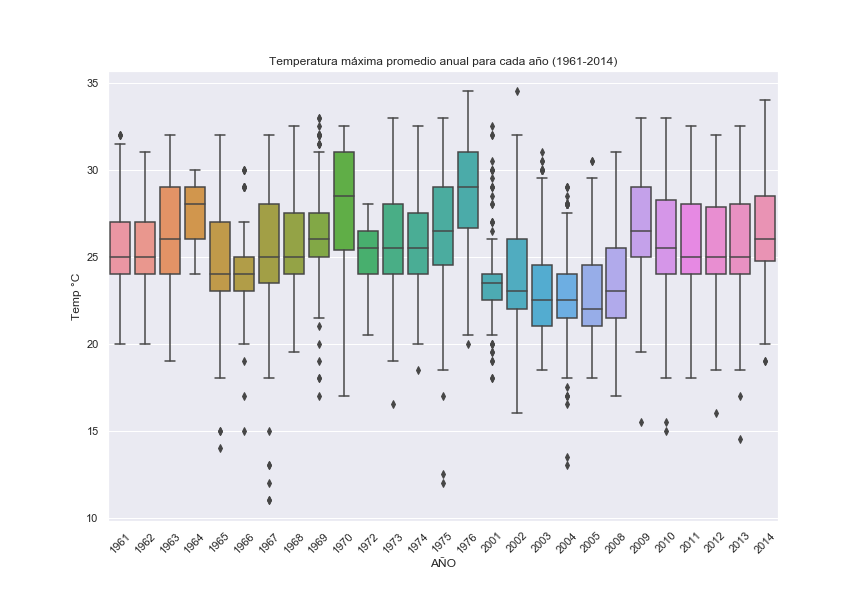
\includegraphics[height=5.3cm]{Temp_promanumax.png}
\end{center}


\section{Conclusiones}
Podemos concluir que la biblioteca Matplotlib y Seaborn son herramientas muy útiles para visualizar datos y realizar un análisis de los mismos a partir de las gráficas, observamos diversos aspectos interesantes del municipio de Valle de Bravo con la información que nos proporciona la correspondiente estación del Servicio Meteorológico Nacional.

\section{Referencias}
\begin{itemize}
\item El Servicio Meteorológico Nacional, Información Estadística Climatológica,\\ Recuperado de:\\ https://smn.cna.gob.mx/es/climatologia/informacion-climatologica/informacion-estadistica-climatologica
\item Matplotlib. Recuperado de:\\ https://matplotlib.org/
\item Seaborn: statistical data visualization. Recuperado de:\\ https://seaborn.pydata.org/generated/seaborn.boxplot.html
\end{itemize}

\end{document}